\documentclass{prova}

\usepackage{amsmath}
\usepackage{amsfonts}

\setlength{\textheight}{25cm}

\renewcommand{\sin}{\,\mbox{sen}\,}
\newcommand{\ds}{\displaystyle}

\professor{Prof.\@ Adriano Barbosa}
\disciplina{C\'alculo Diferencial e Integral}
\avaliacao{P2}
\curso{Engenharia de Produção}
\data{25/05/2021}

\begin{document}
	\cabecalho{5}  % o numero 5 indica a qnt de quadros na tabela de nota

    \textbf{Todas as respostas devem ser justificadas.}

    \begin{questionario}
	    \q{Seja $F(x) = f(2g(3f(x)))$, onde $g(0)=f(0)=0$, $f'(0)=2$ e
	        $g'(0)=1$. Calcule $F'(0)$.}
	    \q{Um balão esférico esvazia de modo que seu raio decresce a uma taxa
            constante de 10 cm/min. A qual taxa o ar está vazando (volume diminui)
            quando o raio do balão é 3 cm?}
        \q{Uma lata que comporta 500 cm$^3$ de óleo é
            fabricada 
            enrolando uma folha retangular de alumínio ao longo do comprimento da borda
            de um disco de alumínio de modo a formar um cilindro sem tampa.
	        Encontre as dimensões (altura e raio) da lata de modo que seja
	        utilizado a menor quantidade possível de material na sua fabricação.}
            \begin{figure}[h]
                \centering
                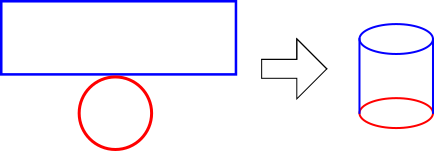
\includegraphics[width=0.4\textwidth]{cilindro.png}
            \end{figure}
	    \q{}
	    	\begin{questionario}
	    		\qq{Calcule $\ds \frac{d}{dx} \int_x^0 \sin(t^2)\ dt$.}
	    		\qq{Calcule a integral $\ds\int_0^\pi \frac{d}{dx}
	    			\left(\cos(x)\sin(x)\right)\ dx$.}
	    		\qq{Qual o valor de $\ds\frac{d}{dx} \int_0^1
	    			\cos(\sin(x^2))\ dx$.}
	    	\end{questionario}
        \q{Determine os valores máximo e mínimo de $f(x)=x-\ln{x}$ no intervalo
            $\ds\left[\frac{1}{2}, 2\right]$.}
    \end{questionario}
\end{document}
